\documentclass{article}

\usepackage{graphicx}
\usepackage{tikz}
\usepackage{tikzsymbols}
\usetikzlibrary{calc,patterns,shapes.geometric}
\pagestyle{empty}
\usepackage[margin=0pt]{geometry}
\geometry{papersize={14in,12in}}

\def\centerarc[#1](#2)(#3:#4:#5){\draw[#1] ($(#2)+({#5*cos(#3)},{#5*sin(#3)})$) arc (#3:#4:#5);}

\begin{document}
	\begin{figure}
		\centering
		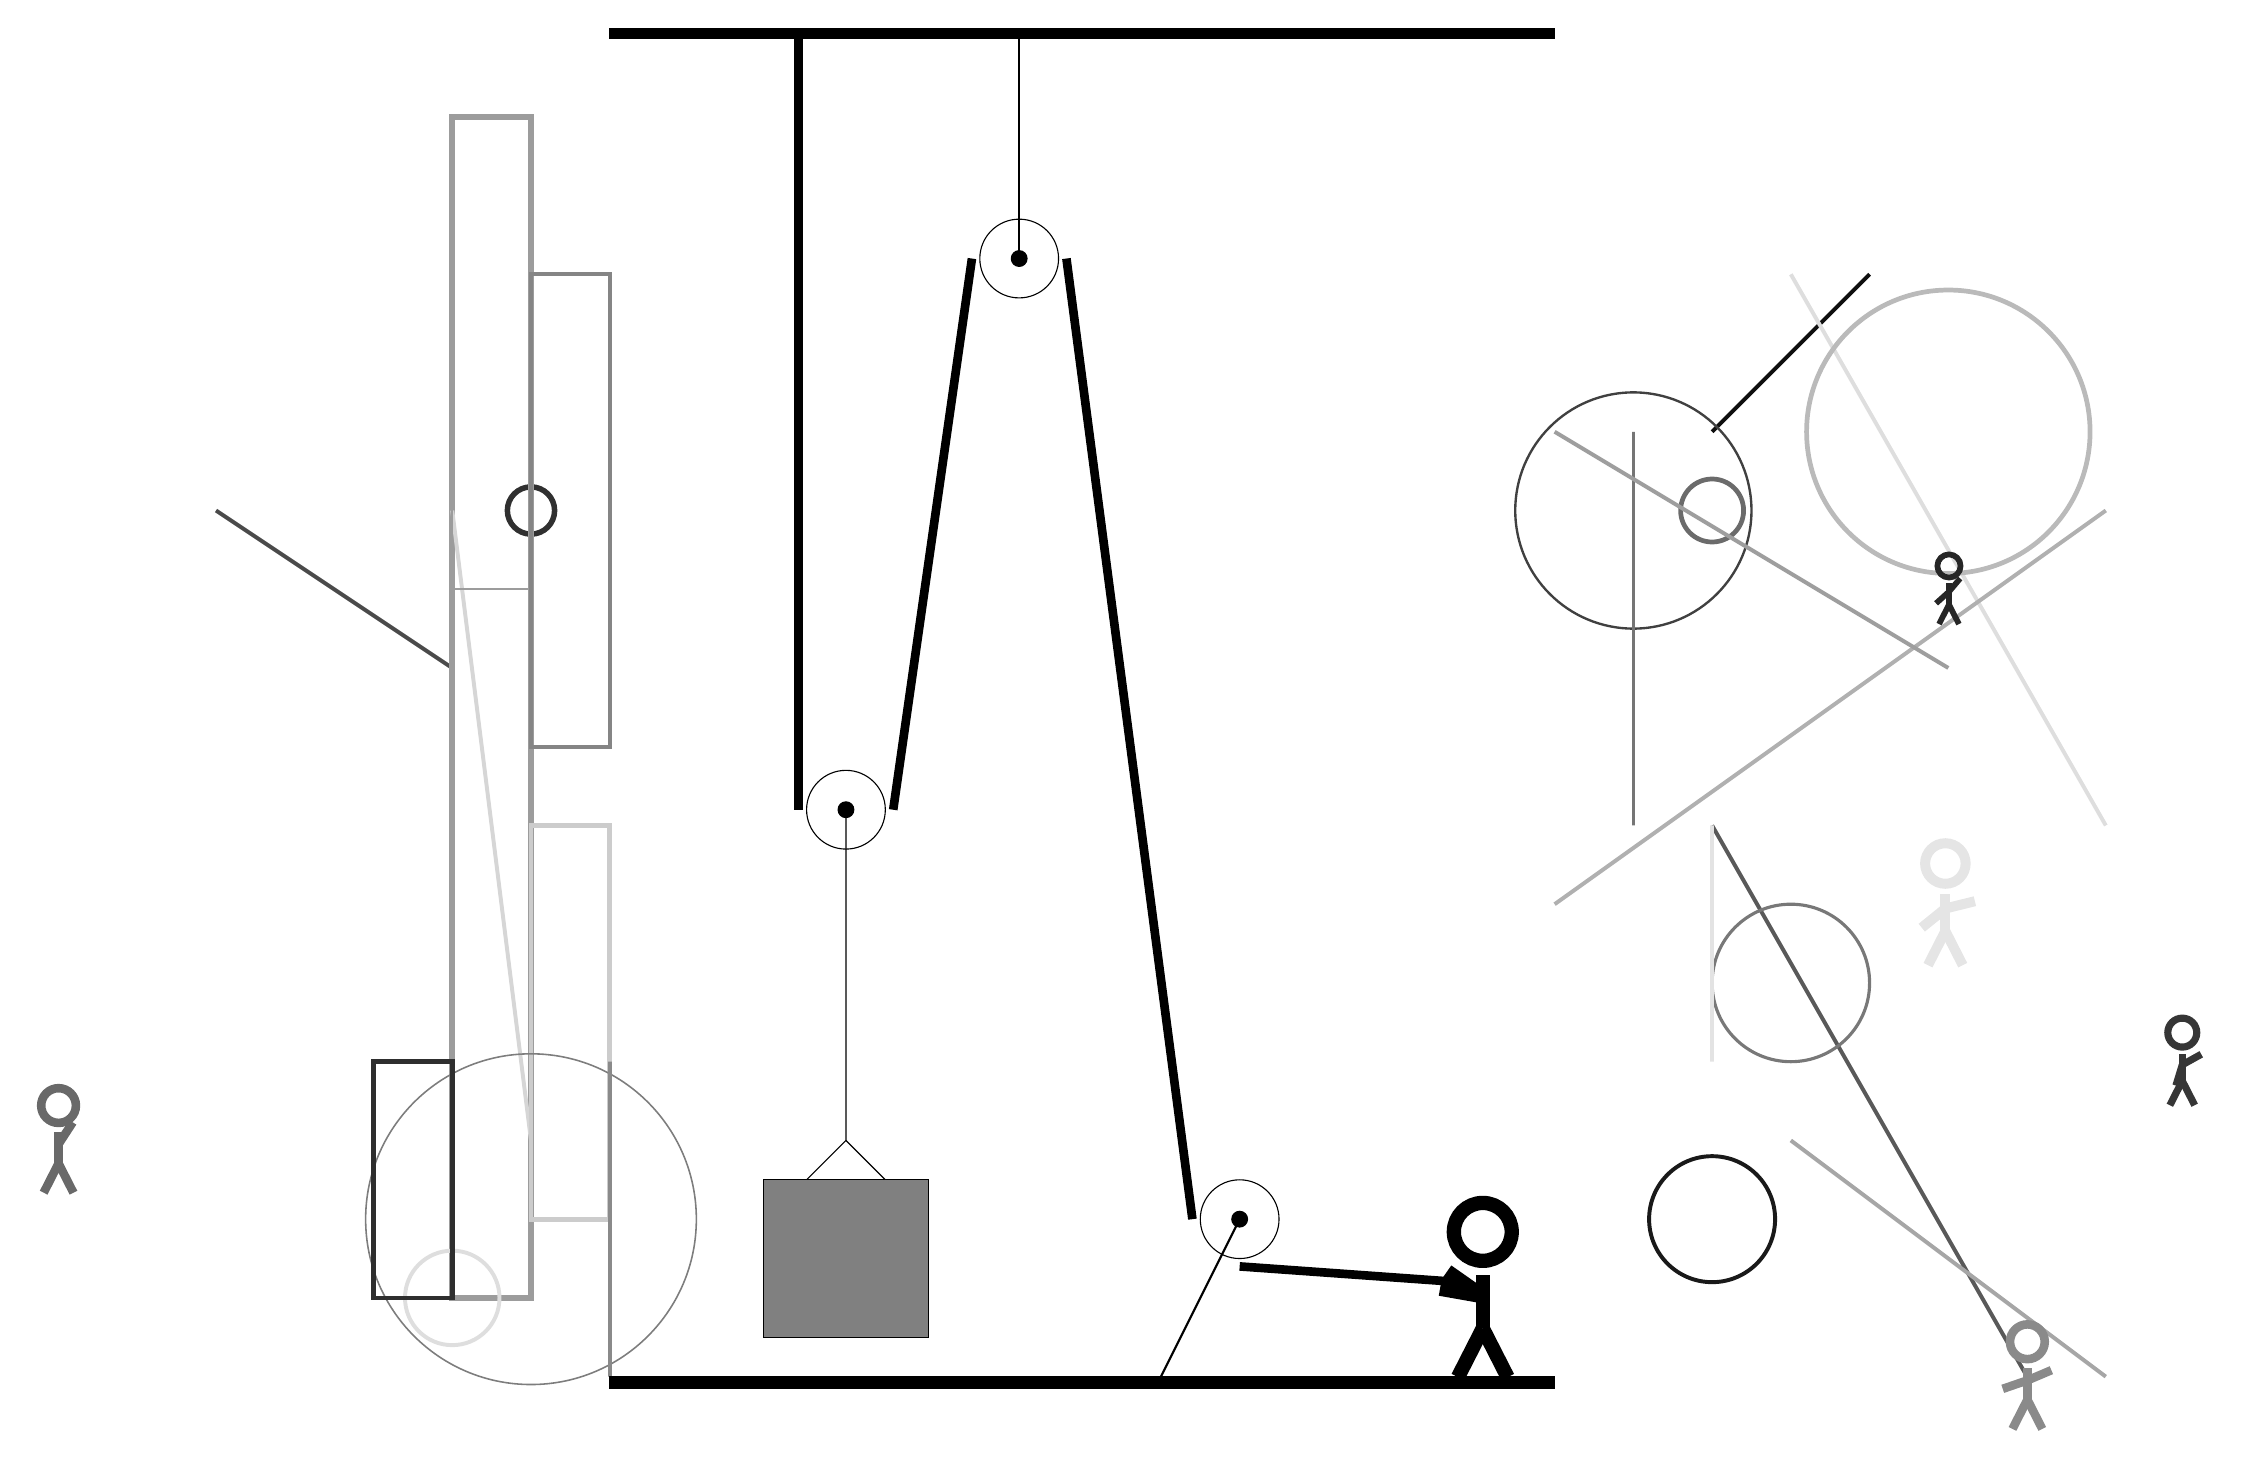
\begin{tikzpicture}
			%%%%% START %%%%%
			
			\draw[fill=black] (-2, 14) rectangle (10, 14.125);
			
			\draw (3.2, 11.2) circle (0.5);
			\draw[fill=black] (3.2, 11.2) circle (0.1);
			\draw[thick] (3.2, 11.2) -- (3.2, 14);
			
			\draw (6, -1) circle (0.5);
			\draw[fill=black] (6, -1) circle (0.1);
			\draw[thick] (6, -1) -- (5, -3);
			
			\draw[line width=0.5mm, color=black!94](14, 11) -- (12, 9);
			
			\draw[line width=0.5mm, color=black!13](13, 11) -- (17, 4);
			\draw[line width=0.5mm, color=black!65](12, 4) -- (16, -3);
			\draw [line width=0.7mm, color=black!81](-3, 8) circle (0.3);
			\draw[line width=0.5mm, color=black!31](10, 3) -- (17, 8);
			\draw [line width=0.3mm, color=black!75](11, 8) circle (1.5);
			\draw[line width=0.5mm, color=black!71](-4, 6) -- (-7, 8);
			\draw [line width=0.6mm, color=black!58](12, 8) circle (0.4);
			\draw [line width=0.4mm, color=black!53](13, 2) circle (1.0);
			\draw[line width=0.7mm, color=black!39] (-3, 13) rectangle (-4, -2);
			\draw[line width=0.5mm, color=black!35](13, 0) -- (17, -3);
			\draw[line width=0.4mm, color=black!54] (11, 9) rectangle (11, 4);
			\node[line width=0.4mm, color=black!10] at (15, 3) {\Strichmaxerl[7][39][14]};
			\draw [line width=0.5mm, color=black!13](-4, -2) circle (0.6);
			\node[line width=0.7mm, color=black!59] at (-9, 0) {\Strichmaxerl[6][90][57]};
			\draw[line width=0.5mm, color=black!38](15, 6) -- (10, 9);
			\draw[line width=0.5mm, color=black!16](-4, 8) -- (-3, 0);
			\draw[line width=0.6mm, color=black!20] (-3, -1) rectangle (-2, 4);
			\draw [line width=0.5mm, color=black!90](12, -1) circle (0.8);
			\draw [line width=0.6mm, color=black!27](15, 9) circle (1.8);
			\node[line width=0.6mm, color=black!46] at (16, -3) {\Strichmaxerl[6][19][23]};
			
			\draw [line width=0.2mm, color=black!51](-3, -1) circle (2.1);
			\node[line width=0.4mm, color=black!85] at (15, 7) {\Strichmaxerl[4][42][50]};
			\draw[line width=0.3mm, color=black!39] (-4, 13) rectangle (-3, 7);
			\draw[line width=0.6mm, color=black!82] (-4, 1) rectangle (-5, -2);
			\node[line width=0.6mm, color=black!79] at (18, 1) {\Strichmaxerl[5][73][29]};
			\draw[line width=0.5mm, color=black!48] (-3, 11) rectangle (-2, 5);
			\draw[line width=0.5mm, color=black!46] (-2, 1) rectangle (-2, -3);
			\draw[line width=0.5mm, color=black!11] (12, 1) rectangle (12, 4);
			
			
			\draw (1, 4.2) circle (0.5);
			\draw[fill=black] (1, 4.2) circle (0.1);
			
			\draw (1, 4.2) -- (1, 0) -- (0.5, -0.5);
			\draw (1, 0) -- (1.5, -0.5);
			\draw[fill=black!50] (-0.05, -0.5) rectangle (2.05, -2.5);
			
			\draw[line width=1.1mm] (0.4, 14) -- (0.4, 4.2);
			\centerarc[line width=1.1mm](1, 4.2)(180:360:0.6);
			\draw[line width=1.1mm](1.6, 4.2) -- (2.6, 11.2);
			\centerarc[line width=1.1mm](3.2, 11.2)(0:180:0.6);
			\draw[line width=1.1mm](3.8, 11.2) -- (5.4, -1);
			\centerarc[line width=1.1mm](6, -1)(180:270:0.6);
			\draw[line width=1.1mm](6, -1.6) -- (8.8, -1.8);
			
			\node at (9, -1.9) {\Strichmaxerl[10][-35][170]};
			
			\draw[fill=black] (-2, -3) rectangle (10, -3.15);
			
			%%%%% END %%%%%
		\end{tikzpicture}
	\end{figure}	
\end{document}